\chapter{Training Loss Curves}
\label{app:loss-curves}

This appendix collects the full-resolution training and evaluation figures referenced in Chapter~4. These plots are provided here so that the main results chapter can remain readable while still preserving the detailed visual evidence used to interpret the model comparison.

The material in this appendix serves two purposes. First, it documents the detailed optimisation behaviour that underpins the summary statistics reported in Section~4.2. Second, it provides additional qualitative examples for the held-out test material so that the waveform- and spectrum-level differences between the two recurrent models can be inspected at a larger scale than is practical in the main chapter.

\section{Per-Model Training Curves}

Figures~\ref{fig:appendix-lstm-loss-curve} and~\ref{fig:appendix-gru-loss-curve} separate the two training runs into full-page views. Presented individually, the curves make it easier to inspect the stability of the validation trajectory, the point at which improvement begins to slow, and the length of the post-best-checkpoint region before early stopping terminates training.

The LSTM curve shows a longer optimisation process with continued gradual validation improvement into the later stages of training, consistent with the lower best-validation loss reported in Table~4.2. By contrast, the GRU curve flattens earlier and reaches its best checkpoint sooner, which supports the interpretation in Chapter~4 that the GRU converged faster but to a less favourable final validation level under the matched training configuration.

\begin{figure}[htbp]
  \centering
  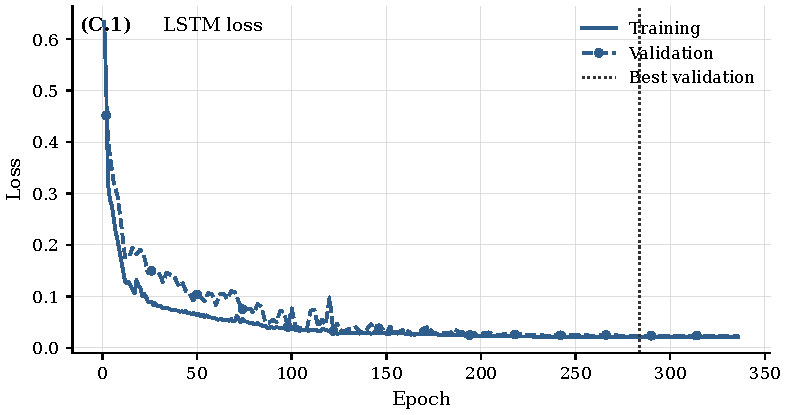
\includegraphics[width=\textwidth]{images/figures/appendix_c_1_lstm_loss_curve.pdf}
  \caption[Full-resolution LSTM loss curves]{Full-resolution LSTM training and validation loss curves.}
  \label{fig:appendix-lstm-loss-curve}
\end{figure}

\begin{figure}[htbp]
  \centering
  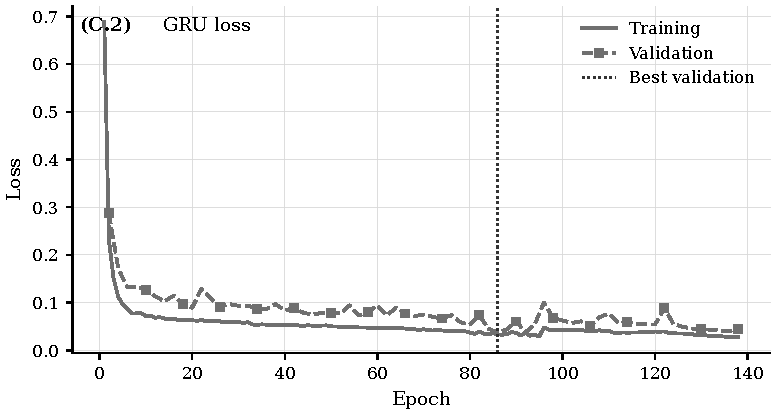
\includegraphics[width=\textwidth]{images/figures/appendix_c_2_gru_loss_curve.pdf}
  \caption[Full-resolution GRU loss curves]{Full-resolution GRU training and validation loss curves.}
  \label{fig:appendix-gru-loss-curve}
\end{figure}

\section{Checkpoint Comparison}

Figure~\ref{fig:appendix-best-vs-final-esr} expands the checkpoint comparison summarised in Table~4.4. Its purpose is to make the reporting decision transparent: the best-validation checkpoint is treated as the primary model state because it represents the parameter set selected by validation performance rather than the arbitrary final epoch reached before early stopping halted training.

The figure also makes the asymmetry between the two architectures easier to see. The LSTM changes very little between the best-validation and final checkpoints, whereas the GRU exhibits a visibly larger increase in ESR at the final checkpoint. This reinforces the conclusion that validation-selected checkpoints are especially important for the GRU under the present training regime.

\begin{figure}[htbp]
  \centering
  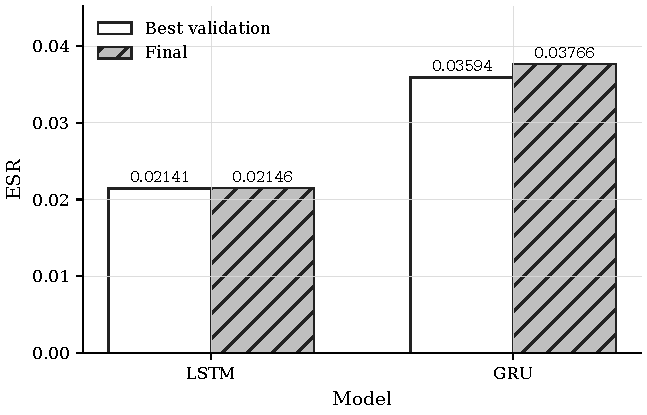
\includegraphics[width=0.9\textwidth]{images/figures/appendix_best_vs_final_esr.pdf}
  \caption[Best-validation and final-checkpoint ESR]{Comparison of best-validation and final-checkpoint ESR for the LSTM and GRU models.}
  \label{fig:appendix-best-vs-final-esr}
\end{figure}

\section{Waveform and Spectral Detail}

The remaining figures provide supplementary qualitative evidence for the objective results reported in Section~4.3. They are not intended to replace the numerical metrics, but to show how the remaining model errors appear in the time and time--frequency domains across more than one excerpt from the held-out test material.

Figures~\ref{fig:appendix-waveform-examples} and~\ref{fig:appendix-spectrogram-examples} extend the single example shown in Chapter~4 by presenting additional waveform and spectrogram views. These examples help distinguish broad agreement in signal shape from the smaller residual differences that remain after training, particularly in transient regions and higher-frequency content.

Figures~\ref{fig:appendix-residual-waveform} and~\ref{fig:appendix-spectral-error} focus directly on the error signal. The residual waveform plots show where the model outputs diverge from the target recording in the time domain, while the spectral-error plot summarises how those differences are distributed across frequency. Read together, these figures provide a fuller visual account of why the LSTM achieved the lower ESR on the held-out test set.

\begin{figure}[htbp]
  \centering
  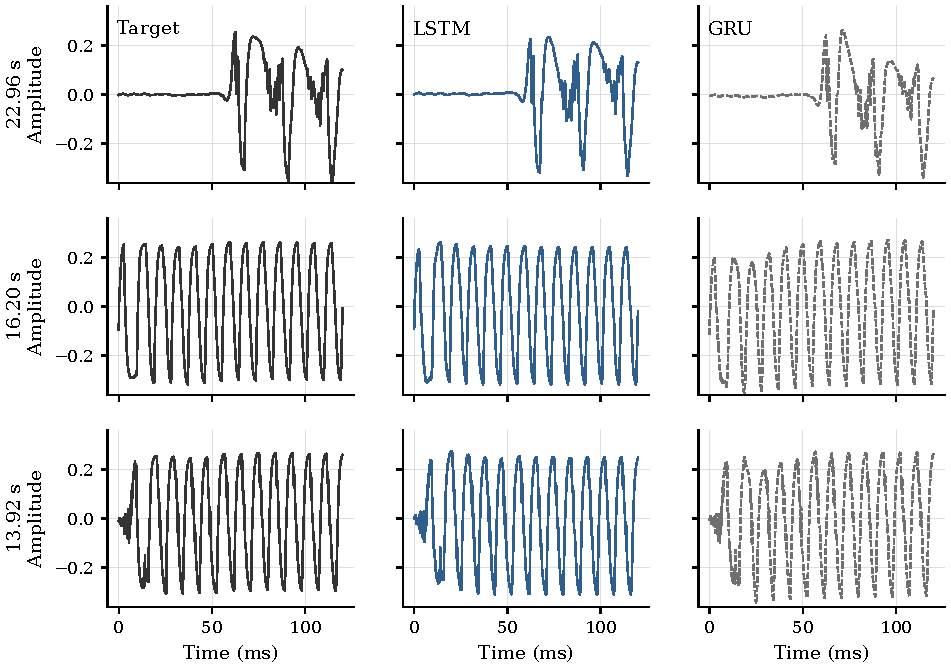
\includegraphics[width=\textwidth]{images/figures/appendix_waveform_examples.pdf}
  \caption[Supplementary waveform comparisons]{Additional waveform comparison examples for the held-out test material.}
  \label{fig:appendix-waveform-examples}
\end{figure}

\begin{figure}[htbp]
  \centering
  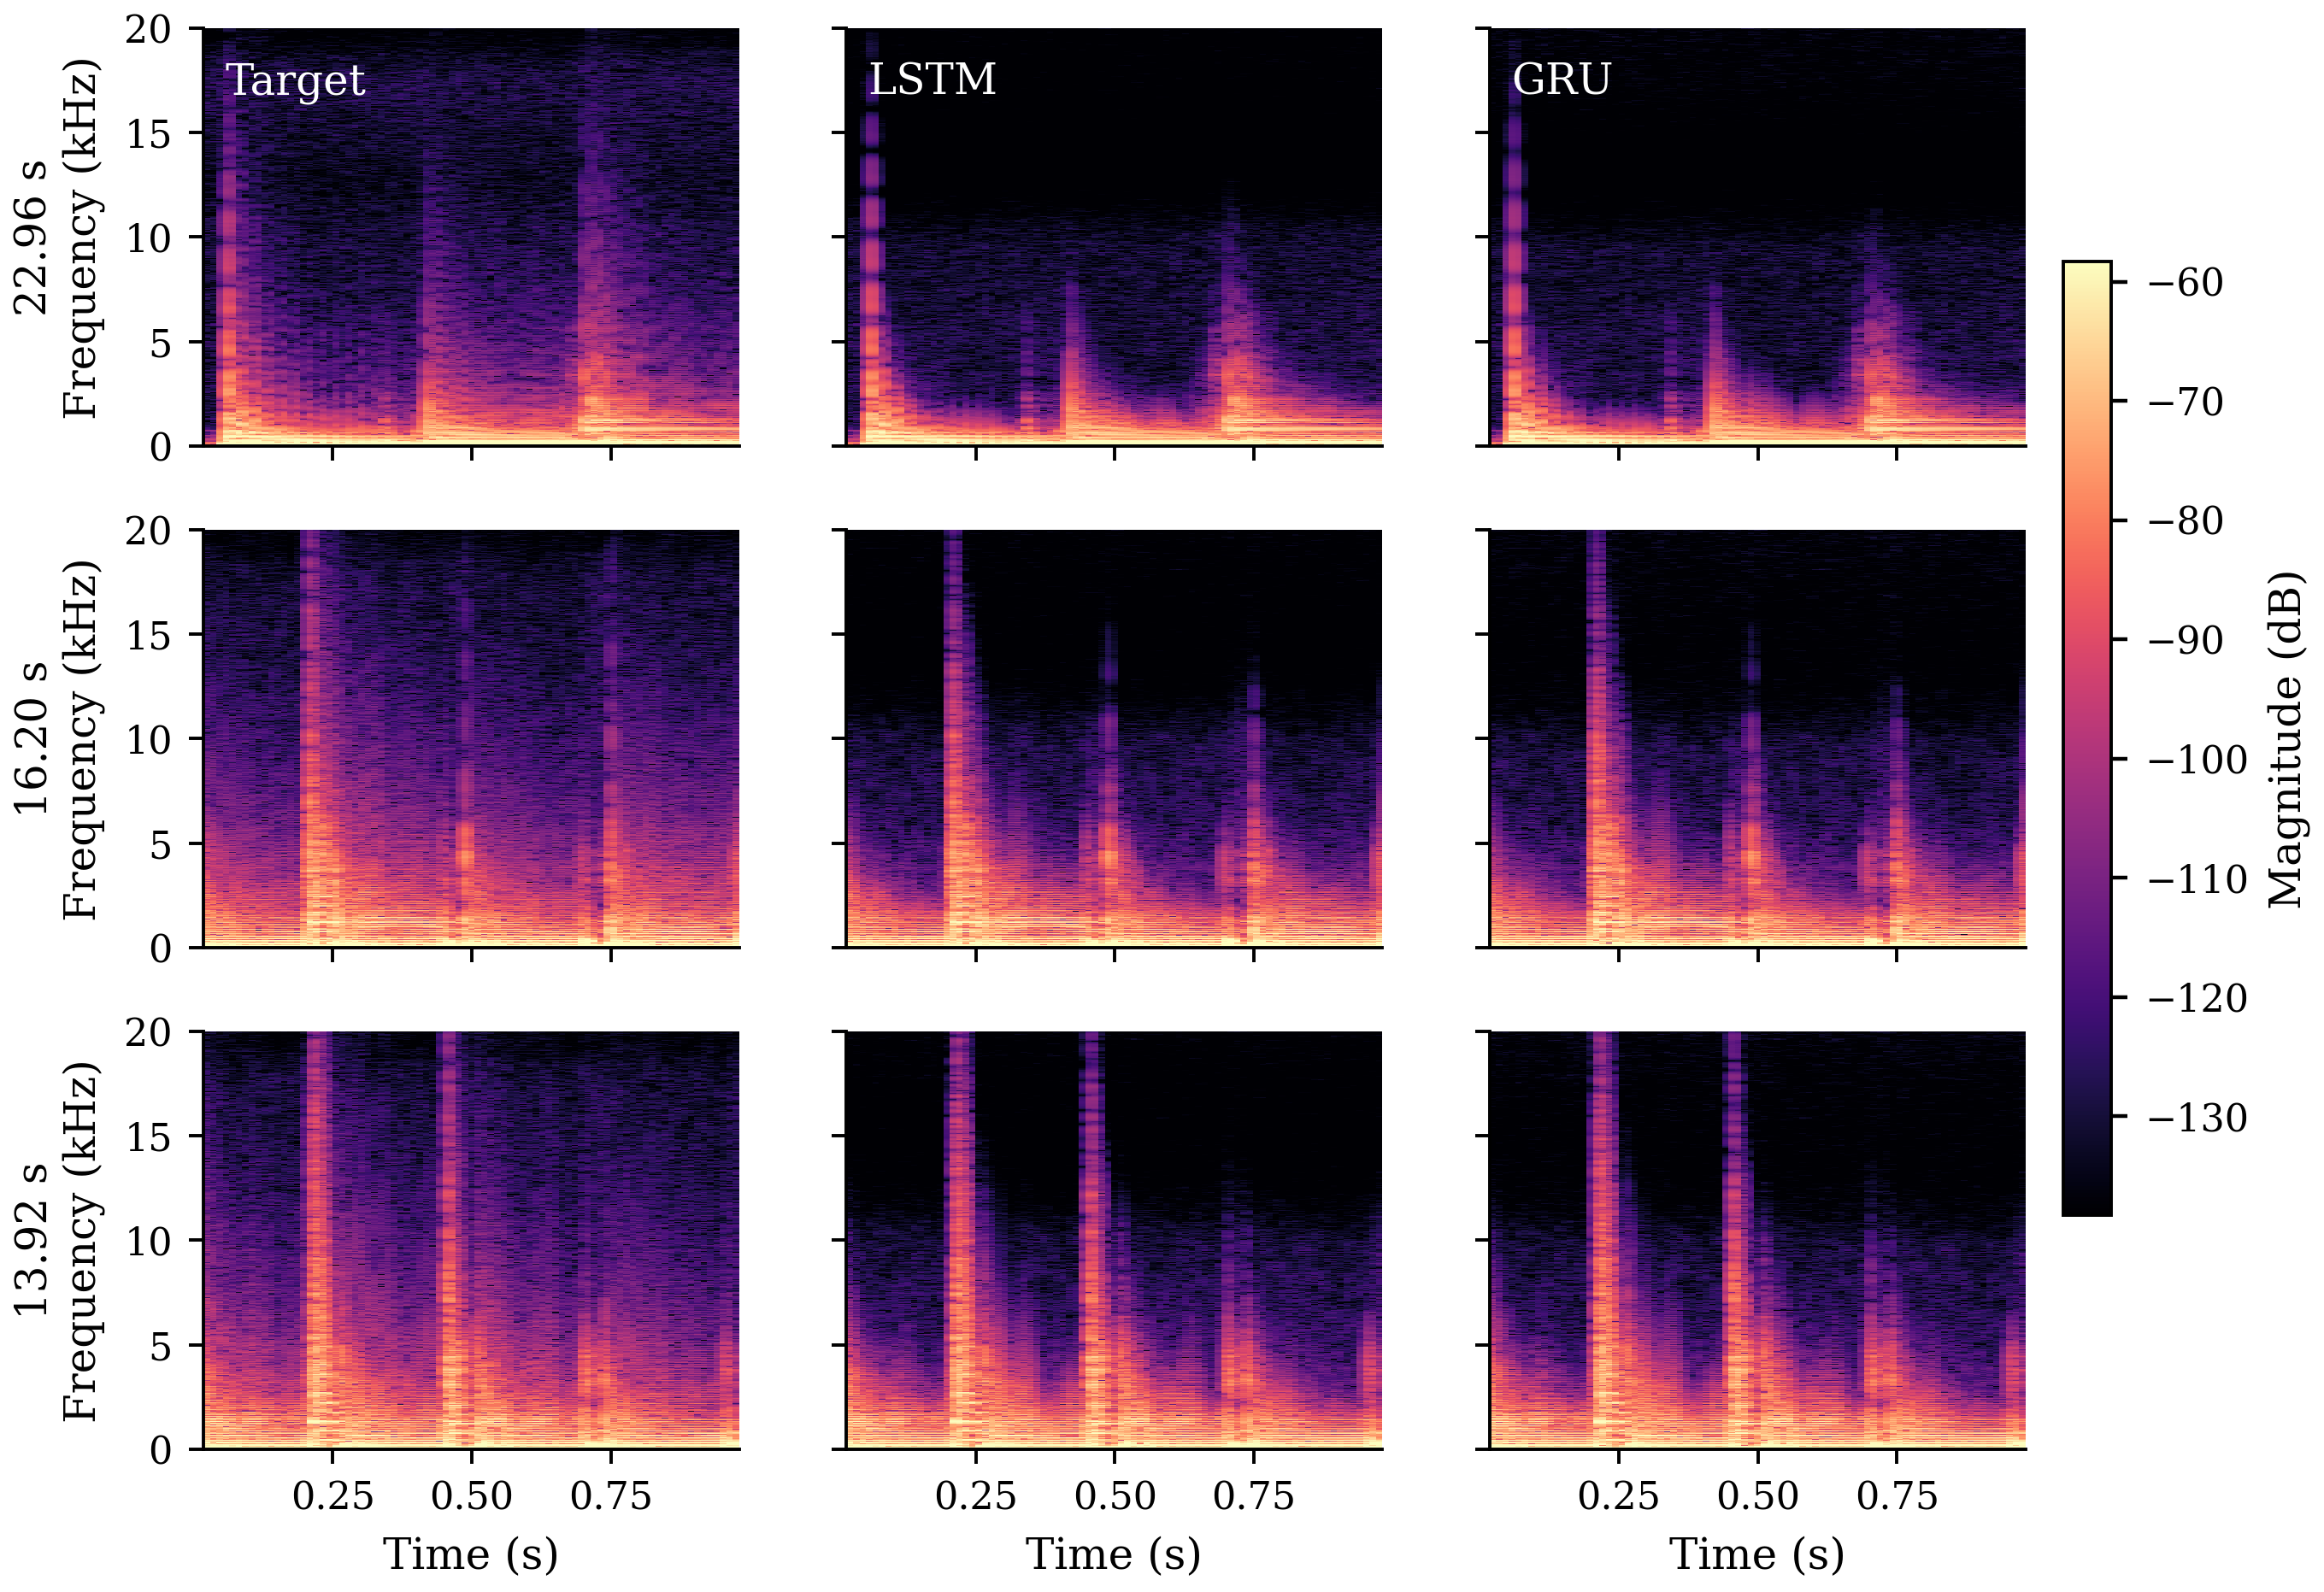
\includegraphics[width=\textwidth]{images/figures/appendix_spectrogram_examples.png}
  \caption[Supplementary spectrogram comparisons]{Additional spectrogram comparison examples for the held-out test material.}
  \label{fig:appendix-spectrogram-examples}
\end{figure}

\begin{figure}[htbp]
  \centering
  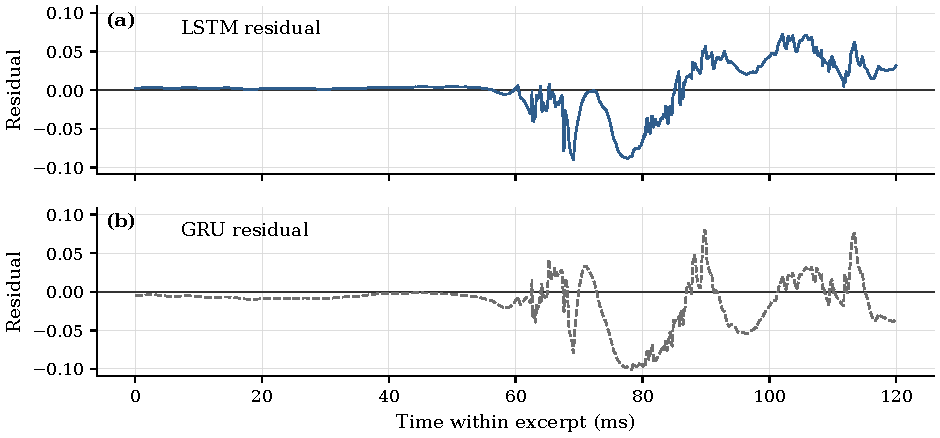
\includegraphics[width=\textwidth]{images/figures/appendix_residual_waveform.pdf}
  \caption[Residual waveform examples]{Residual waveform examples showing the difference between model output and target signal.}
  \label{fig:appendix-residual-waveform}
\end{figure}

\begin{figure}[htbp]
  \centering
  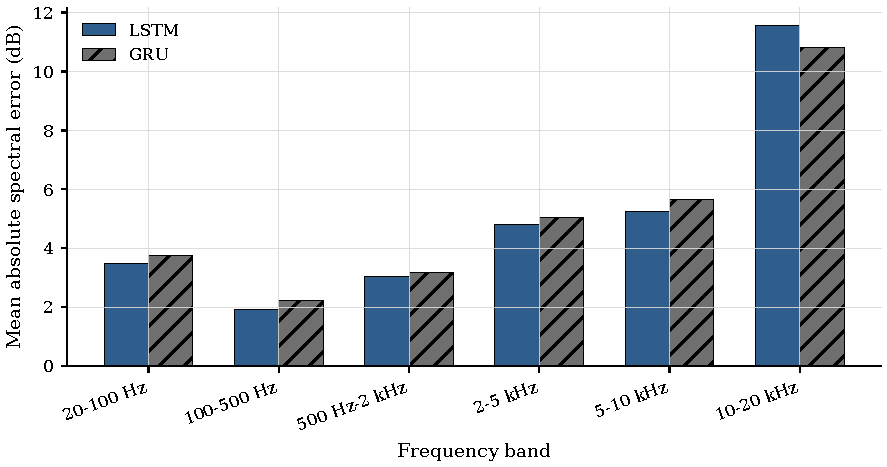
\includegraphics[width=\textwidth]{images/figures/appendix_spectral_error.pdf}
  \caption[Spectral error comparison]{Spectral error comparison across the supplementary test examples.}
  \label{fig:appendix-spectral-error}
\end{figure}
